\documentclass[11pt,a4paper]{article}
\usepackage[utf8]{inputenc}
\usepackage[T1]{fontenc}
\usepackage{lmodern}
\usepackage{booktabs}
\usepackage{graphicx}
\usepackage{caption}
\usepackage{subcaption}
\usepackage{geometry}
\usepackage{xcolor}
\usepackage{float}
\usepackage{graphicx}
\usepackage[table]{xcolor}
\usepackage{rotating}
\definecolor{lightgreen}{RGB}{180,255,180}

\geometry{margin=2cm}

\title{TCPD Benchmark: Comprehensive Comparison of Change Point Detection Methods}
\author{MICA Analysis (using paper-extracted tables)}
\date{\today}

\begin{document}

\maketitle

\section{Introduction}

This document presents a comparison of change point detection methods on the
van den Burg \& Williams (2020) TCPD benchmark suite. Baseline numbers are taken
from the extracted paper tables (Table 2 and per-dataset tables). MICA-O and MICA-P
are recomputed with level continuity across detected changepoints. The analysis uses all 42 TCPD datasets. Baseline numbers come from the paper's extracted per-dataset tables; MICA-O and MICA-P are recomputed with level continuity across detected changepoints on the same 42 datasets. HMM-Regime is run with the same protocol and added as a reviewer-suggested model-based competitor. Means in the bar charts and per-dataset tables are computed over these same 42 datasets, so all methods are compared on identical data. Runs marked as failed/unsupported (``F'', ``M'', or blank) in the paper tables are treated as 0.0 when computing per-method means, so a method that cannot run on a dataset is penalized equally.

\section{Methods Compared}

The following methods from the TCPD paper are included:
\begin{itemize}
    \item \textbf{Paper baselines:} AMOC, BinSeg, BOCPD, BOCPDMS, CPNP, ECP, KernelCPD (KCPA), PELT, PROPHET, RBOCPDMS, RFPOP, SegNeigh, WBS, ZERO
    \item \textbf{Additional baseline:} HMM-Regime (reviewer-suggested model-based competitor)
    \item \textbf{MICA-O:} Model-Informed Change-point Analysis with oracle (best-case) model and penalty selection, with level continuity across segments
    \item \textbf{MICA-P:} Model-Informed Change-point Analysis with practical (automated) BIC-based selection, with level continuity across segments
\end{itemize}

\section{Oracle vs.\ Practical Selection}

The benchmark distinguishes two evaluation modes:

\begin{description}
    \item[With oracle] The true changepoint labels are used to select the best configuration per dataset. This gives an upper-bound: it answers ``how well could a method perform if its model, penalty, and hyperparameters were perfectly tuned?'' For the paper baselines, the oracle numbers come from running each method with many hyperparameter/model variants and keeping the best. For MICA-O, we select the best MICA model, objective, penalty, $\kappa$, \texttt{min\_seg}, and \texttt{step} per dataset using the known labels.
    \item[Without oracle (default/practical)] Only the observed time series is available. The method must use its default settings or an automated criterion to choose its configuration. For the paper baselines, these are the default-setting results. For MICA-P, we use the BIC-based selection criterion (no peeking at the true changepoints).
\end{description}

MICA-O is therefore compared against the baselines' oracle results, and MICA-P against the baselines' default results. The practical--oracle gap for MICA is small, which indicates that the level continuity enforcement and the BIC selector capture most of MICA's best-case performance.

\section{Summary of Mean Performance}

\begin{figure}[H]
    \centering
    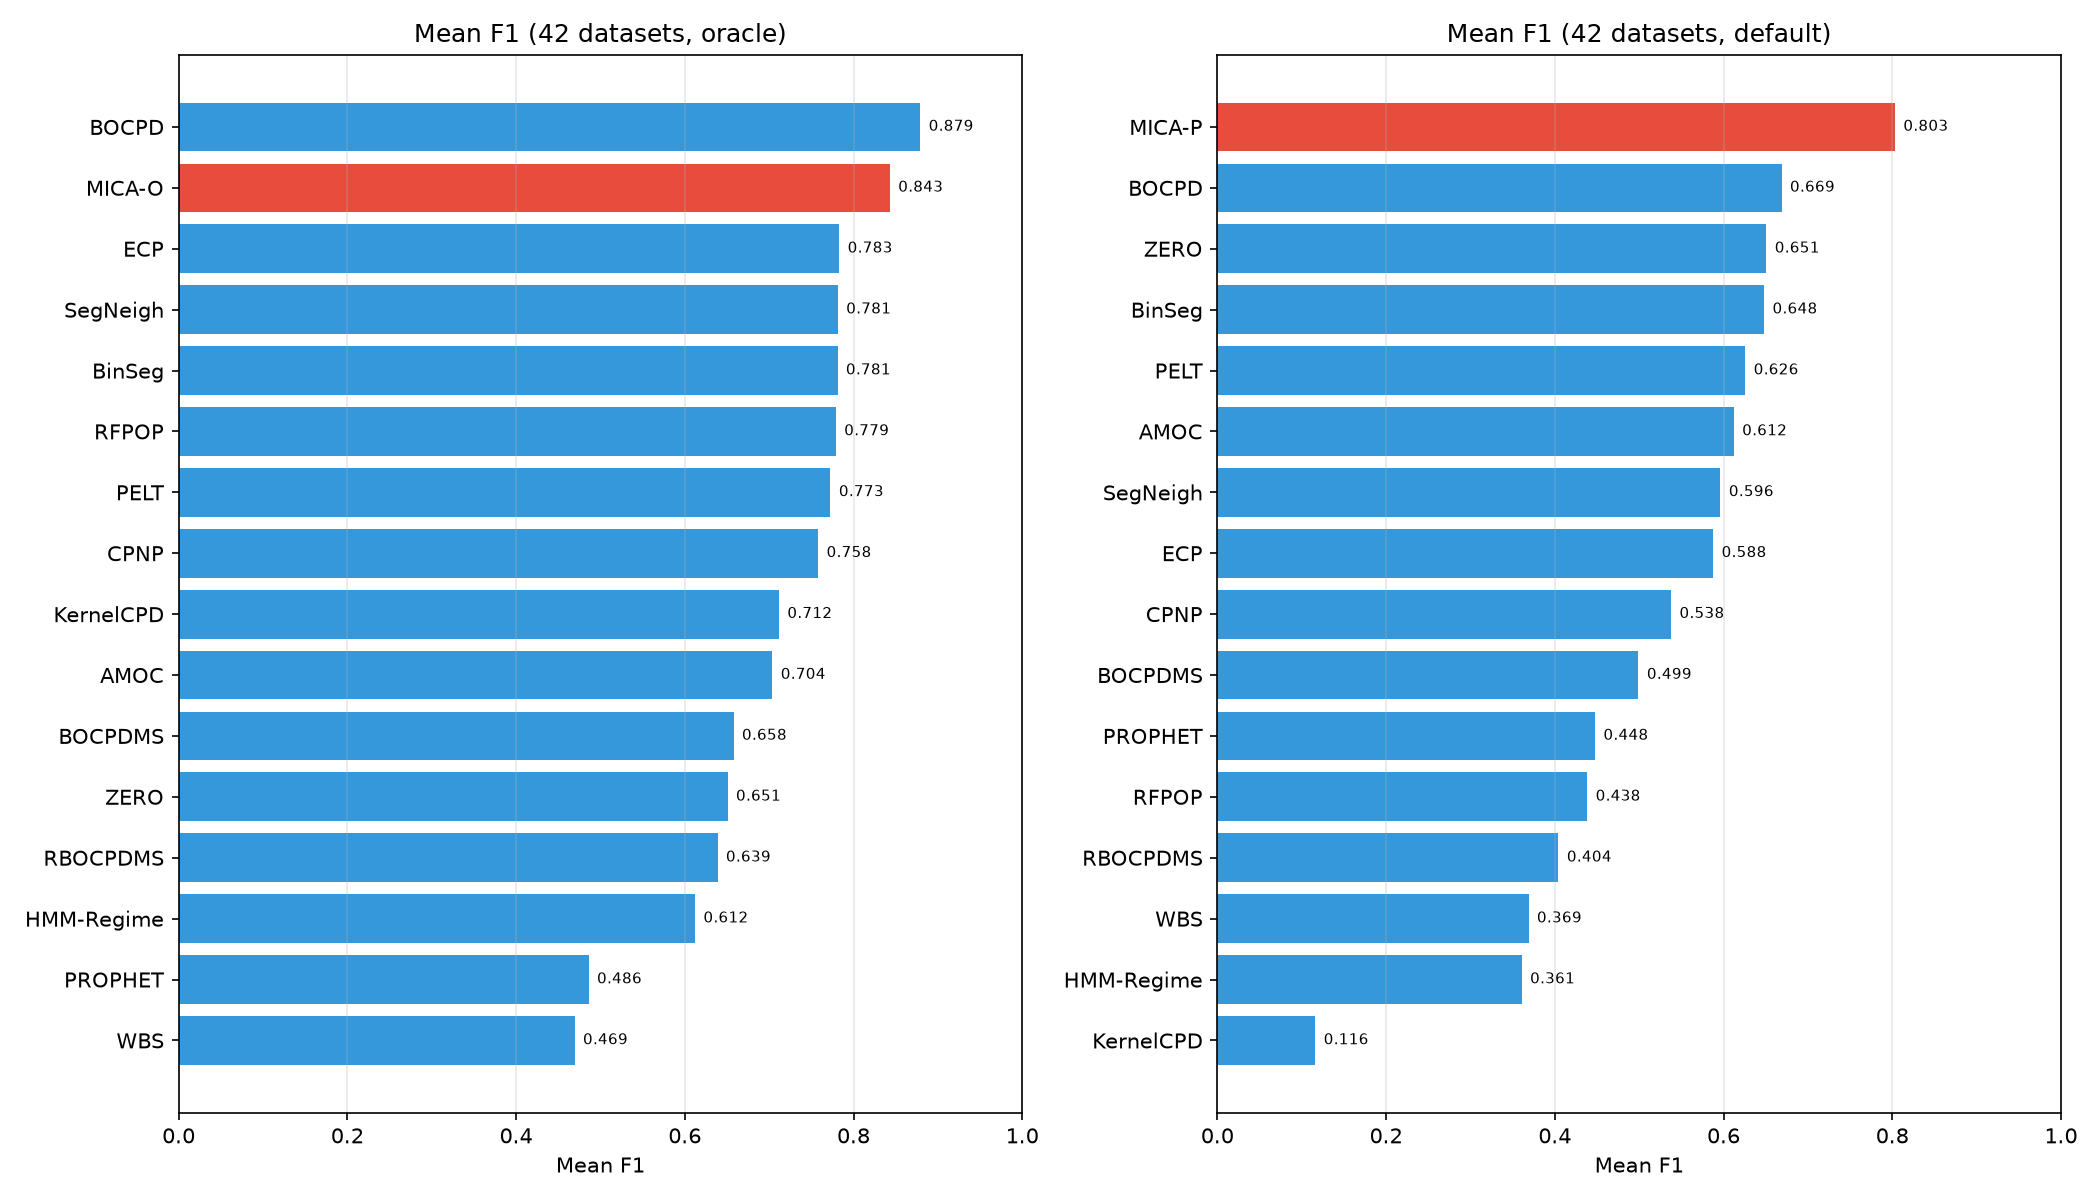
\includegraphics[width=0.95\textwidth]{tcpd_summary_multipanel_continuity.png}
    \caption{Mean F1 score across 42 TCPD datasets for oracle and default/practical selection. MICA variants are highlighted in red.}
    \label{fig:summary-multipanel}
\end{figure}

\clearpage
\begin{sidewaystable}
\centering
\captionof{table}{F1 Score --- Oracle Selection}
\label{tab:f1-oracle}
\setlength{\tabcolsep}{1pt}
\resizebox{\textheight}{!}{%
\begin{tabular}{lcccccccccccccccc}
\toprule
Dataset & AMOC & BinSeg & BOCPD & BOCPDMS & CPNP & ECP & KernelCPD & PELT & PROPHET & RBOCPDMS & RFPOP & SegNeigh & WBS & ZERO & HMM-Regime & MICA \\
\midrule
bank & \textbf{1.000} & \textbf{1.000} & \textbf{1.000} & 0.500 & \textbf{1.000} & 0.200 & 0.333 & \textbf{1.000} & \textbf{1.000} & 0.500 & \textbf{1.000} & \textbf{1.000} & 0.043 & \textbf{1.000} & 0.000 & \textbf{1.000} \\
bitcoin & 0.507 & 0.780 & 0.733 & 0.533 & 0.611 & 0.625 & 0.665 & \textbf{0.783} & 0.446 & 0.422 & 0.727 & \textbf{0.783} & 0.690 & 0.450 & 0.281 & 0.490 \\
brent\_spot & 0.465 & 0.670 & 0.631 & 0.309 & \textbf{0.735} & 0.636 & 0.553 & 0.641 & 0.249 & 0.621 & 0.641 & 0.651 & 0.564 & 0.315 & 0.489 & 0.541 \\
businv & 0.588 & 0.588 & 0.650 & 0.455 & 0.588 & 0.370 & 0.294 & 0.588 & 0.275 & 0.553 & 0.588 & 0.588 & 0.289 & 0.588 & 0.231 & \textbf{0.769} \\
centralia & 0.909 & \textbf{1.000} & \textbf{1.000} & \textbf{1.000} & \textbf{1.000} & 0.909 & \textbf{1.000} & \textbf{1.000} & 0.763 & 0.974 & \textbf{1.000} & \textbf{1.000} & 0.556 & 0.763 & 0.941 & 0.759 \\
children\_per\_woman & 0.678 & 0.678 & 0.787 & 0.826 & 0.734 & 0.551 & 0.525 & 0.778 & 0.310 & 0.580 & 0.637 & 0.778 & 0.500 & 0.507 & 0.286 & \textbf{0.889} \\
co2\_canada & 0.544 & 0.893 & \textbf{0.924} & 0.479 & 0.677 & 0.875 & 0.867 & 0.894 & 0.482 & 0.621 & 0.894 & 0.894 & 0.681 & 0.361 & 0.705 & 0.827 \\
construction & 0.696 & \textbf{0.709} & \textbf{0.709} & 0.516 & \textbf{0.709} & \textbf{0.709} & 0.634 & \textbf{0.709} & 0.324 & 0.615 & \textbf{0.709} & \textbf{0.709} & 0.523 & 0.696 & 0.706 & 0.706 \\
debt\_ireland & 0.760 & \textbf{1.000} & \textbf{1.000} & 0.892 & 0.958 & 0.980 & \textbf{1.000} & \textbf{1.000} & 0.469 & 0.958 & \textbf{1.000} & \textbf{1.000} & 0.538 & 0.469 & 0.947 & 0.947 \\
gdp\_argentina & 0.889 & 0.947 & 0.947 & 0.583 & 0.889 & 0.889 & 0.800 & 0.947 & 0.615 & 0.818 & 0.947 & 0.947 & 0.421 & 0.824 & 0.667 & \textbf{1.000} \\
gdp\_croatia & \textbf{1.000} & 0.824 & \textbf{1.000} & 0.583 & \textbf{1.000} & 0.824 & 0.800 & 0.824 & 0.824 & 0.824 & \textbf{1.000} & 0.824 & 0.167 & 0.824 & 0.667 & \textbf{1.000} \\
gdp\_iran & 0.696 & 0.696 & 0.862 & 0.838 & 0.667 & 0.824 & 0.734 & 0.808 & 0.652 & \textbf{0.899} & 0.833 & 0.808 & 0.576 & 0.652 & 0.571 & 0.800 \\
gdp\_japan & \textbf{1.000} & \textbf{1.000} & \textbf{1.000} & 0.615 & \textbf{1.000} & \textbf{1.000} & 0.500 & \textbf{1.000} & 0.889 & \textbf{1.000} & \textbf{1.000} & \textbf{1.000} & 0.222 & 0.889 & \textbf{1.000} & \textbf{1.000} \\
global\_co2 & \textbf{0.929} & \textbf{0.929} & \textbf{0.929} & 0.458 & 0.846 & \textbf{0.929} & 0.750 & \textbf{0.929} & 0.463 & 0.634 & \textbf{0.929} & \textbf{0.929} & 0.250 & 0.846 & 0.667 & 0.800 \\
homeruns & 0.812 & 0.889 & 0.829 & 0.675 & 0.681 & 0.829 & 0.829 & 0.873 & 0.723 & 0.879 & \textbf{0.961} & 0.873 & 0.664 & 0.659 & 0.783 & 0.756 \\
iceland\_tourism & 0.947 & 0.947 & 0.947 & 0.486 & 0.947 & \textbf{1.000} & 0.486 & 0.947 & 0.220 & 0.667 & 0.947 & 0.947 & 0.200 & 0.947 & 0.000 & 0.667 \\
jfk\_passengers & 0.776 & 0.776 & 0.776 & 0.650 & 0.776 & 0.651 & 0.651 & 0.776 & 0.354 & 0.420 & 0.776 & 0.776 & 0.437 & 0.723 & 0.222 & \textbf{0.933} \\
lga\_passengers & 0.561 & 0.620 & 0.715 & 0.563 & 0.634 & \textbf{0.892} & 0.598 & 0.602 & 0.366 & 0.561 & 0.666 & 0.620 & 0.674 & 0.535 & 0.684 & 0.478 \\
measles & \textbf{0.947} & \textbf{0.947} & \textbf{0.947} & 0.486 & \textbf{0.947} & 0.080 & 0.281 & \textbf{0.947} & 0.391 & 0.090 & \textbf{0.947} & \textbf{0.947} & 0.041 & \textbf{0.947} & 0.083 & 0.667 \\
nile & \textbf{1.000} & \textbf{1.000} & \textbf{1.000} & 0.800 & \textbf{1.000} & \textbf{1.000} & \textbf{1.000} & \textbf{1.000} & 0.824 & 0.800 & \textbf{1.000} & \textbf{1.000} & \textbf{1.000} & 0.824 & \textbf{1.000} & \textbf{1.000} \\
ozone & 0.776 & \textbf{1.000} & 0.966 & 0.778 & \textbf{1.000} & \textbf{1.000} & 0.667 & \textbf{1.000} & 0.723 & \textbf{1.000} & \textbf{1.000} & \textbf{1.000} & 0.286 & 0.723 & 0.667 & \textbf{1.000} \\
rail\_lines & 0.846 & \textbf{0.966} & \textbf{0.966} & 0.889 & \textbf{0.966} & \textbf{0.966} & 0.800 & 0.846 & 0.537 & 0.730 & 0.889 & \textbf{0.966} & 0.205 & 0.537 & 0.947 & 0.824 \\
ratner\_stock & 0.776 & 0.832 & \textbf{0.929} & 0.559 & 0.776 & 0.776 & 0.754 & 0.824 & 0.280 & 0.686 & 0.824 & 0.824 & 0.378 & 0.571 & 0.500 & 0.750 \\
robocalls & 0.800 & \textbf{0.966} & \textbf{0.966} & 0.750 & \textbf{0.966} & \textbf{0.966} & \textbf{0.966} & \textbf{0.966} & 0.636 & 0.765 & \textbf{0.966} & \textbf{0.966} & 0.714 & 0.636 & 0.857 & 0.933 \\
scanline\_126007 & 0.710 & 0.920 & \textbf{0.964} & 0.837 & 0.927 & 0.870 & 0.838 & 0.889 & 0.644 & 0.570 & 0.914 & 0.940 & 0.818 & 0.644 & 0.804 & 0.820 \\
scanline\_42049 & 0.485 & 0.931 & \textbf{0.962} & 0.921 & 0.809 & 0.910 & 0.908 & 0.910 & 0.269 & 0.526 & 0.910 & 0.920 & 0.650 & 0.276 & 0.897 & 0.829 \\
seatbelts & 0.824 & 0.838 & 0.683 & 0.583 & 0.838 & 0.683 & 0.683 & 0.683 & 0.452 & 0.621 & 0.683 & 0.838 & 0.583 & 0.621 & 0.429 & \textbf{1.000} \\
shanghai\_license & \textbf{0.966} & \textbf{0.966} & 0.868 & 0.651 & \textbf{0.966} & 0.868 & 0.465 & \textbf{0.966} & 0.532 & 0.778 & \textbf{0.966} & \textbf{0.966} & 0.385 & 0.636 & 0.486 & 0.947 \\
uk\_coal\_employ & — & — & — & 0.617 & — & 0.513 & 0.513 & — & 0.639 & — & — & — & — & 0.513 & \textbf{0.806} & 0.743 \\
unemployment\_nl & 0.742 & \textbf{0.889} & 0.876 & 0.797 & 0.773 & 0.755 & 0.744 & 0.816 & 0.566 & 0.697 & 0.851 & 0.816 & 0.801 & 0.566 & 0.642 & 0.882 \\
us\_population & \textbf{1.000} & \textbf{1.000} & \textbf{1.000} & 0.615 & 0.947 & 0.471 & 0.276 & \textbf{1.000} & 0.159 & 0.320 & 0.889 & \textbf{1.000} & 0.113 & 0.889 & 0.000 & \textbf{1.000} \\
usd\_isk & 0.785 & 0.785 & 0.876 & 0.678 & 0.785 & 0.785 & 0.601 & 0.785 & 0.489 & 0.881 & 0.785 & 0.785 & 0.636 & 0.489 & 0.824 & \textbf{0.888} \\
well\_log & 0.336 & 0.944 & 0.908 & 0.796 & 0.878 & 0.928 & 0.950 & 0.912 & 0.149 & 0.644 & \textbf{0.966} & 0.912 & 0.832 & 0.237 & 0.676 & 0.595 \\
quality\_control\_1 & \textbf{1.000} & \textbf{1.000} & \textbf{1.000} & 0.667 & \textbf{1.000} & \textbf{1.000} & 0.667 & \textbf{1.000} & 0.500 & 0.667 & \textbf{1.000} & \textbf{1.000} & 0.667 & 0.667 & \textbf{1.000} & \textbf{1.000} \\
quality\_control\_2 & \textbf{1.000} & \textbf{1.000} & \textbf{1.000} & 0.800 & \textbf{1.000} & \textbf{1.000} & \textbf{1.000} & \textbf{1.000} & 0.750 & 0.667 & \textbf{1.000} & \textbf{1.000} & \textbf{1.000} & 0.750 & \textbf{1.000} & \textbf{1.000} \\
quality\_control\_3 & \textbf{1.000} & \textbf{1.000} & \textbf{1.000} & 0.766 & \textbf{1.000} & \textbf{1.000} & \textbf{1.000} & \textbf{1.000} & 0.667 & 0.667 & \textbf{1.000} & \textbf{1.000} & \textbf{1.000} & 0.667 & \textbf{1.000} & \textbf{1.000} \\
quality\_control\_4 & 0.810 & 0.873 & 0.810 & 0.561 & 0.810 & 0.726 & 0.658 & 0.810 & 0.780 & 0.438 & 0.873 & 0.810 & 0.608 & 0.780 & 0.647 & \textbf{0.909} \\
quality\_control\_5 & \textbf{1.000} & \textbf{1.000} & \textbf{1.000} & 0.500 & \textbf{1.000} & \textbf{1.000} & \textbf{1.000} & \textbf{1.000} & \textbf{1.000} & 0.500 & \textbf{1.000} & \textbf{1.000} & \textbf{1.000} & \textbf{1.000} & 0.000 & \textbf{1.000} \\
apple & — & — & 0.916 & 0.552 & — & 0.745 & 0.634 & — & — & 0.575 & — & — & — & 0.594 & 0.636 & \textbf{0.919} \\
bee\_waggle\_6 & — & — & \textbf{0.929} & 0.651 & — & 0.233 & 0.651 & — & — & 0.359 & — & — & — & \textbf{0.929} & 0.250 & 0.667 \\
occupancy & — & — & 0.919 & 0.714 & — & \textbf{0.932} & 0.812 & — & — & 0.605 & — & — & — & 0.341 & 0.764 & 0.915 \\
run\_log & — & — & \textbf{1.000} & 0.698 & — & 0.990 & \textbf{1.000} & — & — & 0.698 & — & — & — & 0.446 & 0.947 & 0.756 \\
\midrule
\textbf{Mean} & \textbf{0.704} & \textbf{0.781} & \textbf{0.879} & \textbf{0.658} & \textbf{0.758} & \textbf{0.783} & \textbf{0.712} & \textbf{0.773} & \textbf{0.486} & \textbf{0.639} & \textbf{0.779} & \textbf{0.781} & \textbf{0.469} & \textbf{0.651} & \textbf{0.612} & \textbf{0.843} \\
\bottomrule
\end{tabular}%
}
\end{sidewaystable}
\clearpage

\clearpage
\begin{sidewaystable}
\centering
\captionof{table}{F1 Score --- Default / Practical Selection}
\label{tab:f1-practical}
\setlength{\tabcolsep}{1pt}
\resizebox{\textheight}{!}{%
\begin{tabular}{lcccccccccccccccc}
\toprule
Dataset & AMOC & BinSeg & BOCPD & BOCPDMS & CPNP & ECP & KernelCPD & PELT & PROPHET & RBOCPDMS & RFPOP & SegNeigh & WBS & ZERO & HMM-Regime & MICA \\
\midrule
bank & 0.667 & 0.400 & 0.047 & 0.118 & 0.044 & 0.154 & 0.008 & 0.400 & 0.154 & 0.286 & 0.015 & 0.333 & 0.039 & \textbf{1.000} & 0.000 & \textbf{1.000} \\
bitcoin & 0.367 & 0.426 & \textbf{0.692} & 0.269 & 0.463 & 0.338 & 0.092 & 0.672 & 0.446 & — & 0.284 & 0.672 & 0.464 & 0.450 & 0.051 & 0.447 \\
brent\_spot & 0.272 & 0.483 & 0.521 & 0.239 & \textbf{0.607} & 0.478 & 0.104 & 0.465 & 0.249 & 0.321 & 0.490 & 0.431 & 0.516 & 0.315 & 0.489 & 0.503 \\
businv & 0.455 & 0.370 & 0.270 & 0.370 & 0.304 & 0.301 & 0.047 & 0.370 & 0.275 & 0.238 & 0.245 & 0.312 & 0.230 & 0.588 & 0.000 & \textbf{0.769} \\
centralia & 0.763 & 0.909 & 0.909 & 0.846 & 0.909 & 0.763 & 0.714 & 0.909 & 0.763 & 0.846 & \textbf{1.000} & 0.909 & 0.556 & 0.763 & 0.941 & 0.759 \\
children\_per\_woman & 0.618 & 0.618 & 0.637 & 0.337 & 0.326 & 0.349 & 0.068 & 0.618 & 0.310 & 0.432 & 0.246 & 0.337 & 0.271 & 0.507 & 0.091 & \textbf{0.889} \\
co2\_canada & 0.544 & 0.691 & 0.619 & 0.265 & 0.578 & 0.817 & 0.169 & 0.661 & 0.482 & 0.381 & 0.569 & 0.661 & 0.520 & 0.361 & 0.121 & \textbf{0.827} \\
construction & 0.516 & \textbf{0.709} & 0.634 & 0.410 & 0.602 & 0.574 & 0.038 & \textbf{0.709} & 0.324 & 0.291 & 0.185 & \textbf{0.709} & 0.316 & 0.696 & 0.273 & 0.600 \\
debt\_ireland & 0.469 & 0.760 & 0.760 & 0.611 & 0.760 & 0.469 & 0.519 & 0.760 & 0.469 & 0.530 & 0.824 & 0.760 & 0.538 & 0.469 & 0.621 & \textbf{0.947} \\
gdp\_argentina & 0.889 & 0.889 & 0.947 & 0.583 & 0.818 & 0.824 & 0.131 & 0.889 & 0.615 & 0.452 & 0.571 & 0.947 & 0.148 & 0.824 & 0.400 & \textbf{1.000} \\
gdp\_croatia & 0.583 & 0.583 & \textbf{1.000} & 0.583 & \textbf{1.000} & 0.824 & 0.160 & 0.583 & 0.824 & 0.452 & 0.400 & 0.583 & 0.167 & 0.824 & 0.000 & \textbf{1.000} \\
gdp\_iran & 0.492 & 0.492 & 0.622 & 0.492 & 0.330 & 0.652 & 0.219 & 0.492 & 0.652 & 0.395 & 0.609 & 0.395 & 0.246 & 0.652 & 0.000 & \textbf{0.772} \\
gdp\_japan & 0.615 & 0.615 & 0.800 & 0.471 & 0.667 & 0.889 & 0.068 & 0.615 & 0.889 & 0.471 & 0.190 & 0.615 & 0.077 & 0.889 & 0.667 & \textbf{1.000} \\
global\_co2 & \textbf{0.929} & \textbf{0.929} & 0.754 & 0.458 & 0.421 & 0.754 & 0.167 & 0.754 & 0.463 & 0.458 & 0.293 & 0.754 & 0.179 & 0.846 & 0.000 & 0.800 \\
homeruns & \textbf{0.812} & \textbf{0.812} & 0.729 & 0.552 & 0.604 & 0.675 & 0.133 & \textbf{0.812} & 0.723 & 0.508 & 0.661 & 0.397 & 0.593 & 0.659 & 0.067 & 0.756 \\
iceland\_tourism & 0.643 & 0.643 & 0.486 & 0.391 & 0.391 & 0.391 & 0.021 & 0.643 & 0.220 & 0.667 & 0.200 & 0.486 & 0.200 & \textbf{0.947} & 0.000 & 0.667 \\
jfk\_passengers & 0.776 & 0.776 & 0.437 & 0.559 & 0.574 & 0.437 & 0.026 & 0.776 & 0.354 & 0.296 & 0.344 & 0.650 & 0.437 & 0.723 & 0.153 & \textbf{0.857} \\
lga\_passengers & 0.422 & 0.438 & \textbf{0.630} & 0.297 & 0.606 & 0.392 & 0.054 & 0.438 & 0.366 & 0.348 & 0.498 & 0.395 & 0.524 & 0.535 & 0.383 & 0.419 \\
measles & \textbf{0.947} & \textbf{0.947} & 0.069 & 0.124 & 0.118 & 0.069 & 0.004 & 0.124 & 0.391 & 0.117 & 0.030 & 0.327 & 0.039 & \textbf{0.947} & 0.000 & 0.000 \\
nile & \textbf{1.000} & \textbf{1.000} & \textbf{1.000} & 0.800 & \textbf{1.000} & \textbf{1.000} & 0.040 & \textbf{1.000} & 0.824 & 0.452 & \textbf{1.000} & \textbf{1.000} & \textbf{1.000} & 0.824 & 0.333 & \textbf{1.000} \\
ozone & 0.531 & 0.650 & 0.650 & 0.531 & 0.750 & 0.723 & 0.109 & \textbf{1.000} & 0.723 & 0.559 & 0.375 & \textbf{1.000} & 0.113 & 0.723 & 0.636 & \textbf{1.000} \\
rail\_lines & 0.846 & 0.846 & 0.846 & 0.349 & \textbf{0.966} & 0.537 & 0.200 & 0.846 & 0.423 & 0.349 & 0.571 & 0.846 & 0.205 & 0.537 & 0.947 & 0.824 \\
ratner\_stock & 0.776 & \textbf{0.824} & 0.783 & 0.500 & 0.306 & 0.282 & 0.034 & 0.650 & 0.280 & 0.559 & 0.203 & \textbf{0.824} & 0.250 & 0.571 & 0.444 & 0.750 \\
robocalls & 0.800 & 0.800 & \textbf{0.966} & 0.696 & 0.832 & 0.636 & 0.179 & 0.800 & 0.636 & 0.593 & 0.714 & \textbf{0.966} & 0.182 & 0.636 & 0.857 & 0.933 \\
scanline\_126007 & 0.710 & 0.739 & 0.820 & 0.718 & \textbf{0.889} & 0.732 & 0.101 & 0.759 & 0.644 & — & 0.649 & 0.732 & 0.616 & 0.644 & 0.804 & 0.820 \\
scanline\_42049 & 0.485 & 0.713 & \textbf{0.962} & 0.844 & 0.705 & 0.580 & 0.164 & 0.804 & 0.269 & 0.390 & 0.460 & 0.748 & 0.571 & 0.276 & 0.843 & 0.829 \\
seatbelts & 0.474 & 0.683 & 0.583 & 0.383 & 0.509 & 0.321 & 0.051 & 0.683 & 0.452 & 0.383 & 0.494 & 0.583 & 0.583 & 0.621 & 0.240 & \textbf{0.957} \\
shanghai\_license & 0.868 & 0.868 & 0.713 & 0.491 & 0.437 & 0.698 & 0.048 & 0.868 & 0.532 & 0.326 & 0.357 & 0.713 & 0.208 & 0.636 & 0.486 & \textbf{0.947} \\
uk\_coal\_employ & — & — & — & 0.495 & — & 0.513 & 0.513 & — & 0.639 & — & — & — & — & 0.513 & 0.528 & \textbf{0.743} \\
unemployment\_nl & 0.566 & 0.876 & 0.683 & 0.592 & 0.683 & 0.620 & 0.145 & 0.773 & 0.566 & 0.495 & 0.549 & 0.773 & 0.571 & 0.566 & 0.396 & \textbf{0.882} \\
us\_population & \textbf{1.000} & 0.667 & 0.216 & 0.471 & 0.216 & 0.174 & 0.007 & 0.471 & 0.159 & 0.320 & 0.889 & 0.320 & 0.077 & 0.889 & 0.000 & 0.500 \\
usd\_isk & 0.785 & 0.657 & 0.609 & 0.678 & 0.504 & 0.661 & 0.079 & 0.657 & 0.489 & 0.282 & 0.390 & 0.657 & 0.513 & 0.489 & 0.405 & \textbf{0.888} \\
well\_log & 0.279 & 0.534 & 0.796 & 0.797 & 0.822 & 0.818 & 0.069 & 0.555 & 0.149 & 0.517 & \textbf{0.923} & 0.485 & 0.724 & 0.237 & 0.591 & 0.549 \\
quality\_control\_1 & \textbf{1.000} & \textbf{1.000} & 0.800 & 0.667 & 0.667 & 0.667 & 0.025 & \textbf{1.000} & 0.500 & 0.667 & 0.667 & \textbf{1.000} & 0.571 & 0.667 & 0.667 & \textbf{1.000} \\
quality\_control\_2 & \textbf{1.000} & \textbf{1.000} & \textbf{1.000} & 0.667 & \textbf{1.000} & \textbf{1.000} & 0.028 & \textbf{1.000} & 0.545 & 0.667 & \textbf{1.000} & \textbf{1.000} & \textbf{1.000} & 0.750 & 0.250 & \textbf{1.000} \\
quality\_control\_3 & \textbf{1.000} & \textbf{1.000} & \textbf{1.000} & 0.667 & 0.571 & \textbf{1.000} & 0.022 & \textbf{1.000} & 0.667 & 0.667 & 0.286 & \textbf{1.000} & \textbf{1.000} & 0.667 & 0.143 & \textbf{1.000} \\
quality\_control\_4 & 0.810 & \textbf{0.873} & 0.658 & 0.438 & 0.608 & 0.393 & 0.028 & 0.726 & 0.335 & 0.360 & 0.233 & 0.726 & 0.246 & 0.780 & 0.220 & 0.857 \\
quality\_control\_5 & \textbf{1.000} & \textbf{1.000} & \textbf{1.000} & 0.500 & \textbf{1.000} & \textbf{1.000} & 0.006 & \textbf{1.000} & \textbf{1.000} & 0.500 & \textbf{1.000} & \textbf{1.000} & \textbf{1.000} & \textbf{1.000} & 0.000 & \textbf{1.000} \\
apple & — & — & 0.513 & 0.382 & — & 0.513 & 0.029 & — & — & 0.239 & — & — & — & 0.594 & 0.636 & \textbf{0.904} \\
bee\_waggle\_6 & — & — & 0.121 & 0.388 & — & 0.124 & 0.010 & — & — & 0.179 & — & — & — & \textbf{0.929} & 0.000 & 0.667 \\
occupancy & — & — & 0.807 & 0.461 & — & 0.750 & 0.107 & — & — & 0.329 & — & — & — & 0.341 & 0.629 & \textbf{0.915} \\
run\_log & — & — & \textbf{1.000} & 0.475 & — & 0.792 & 0.139 & — & — & 0.660 & — & — & — & 0.446 & 0.837 & 0.756 \\
\midrule
\textbf{Mean} & \textbf{0.612} & \textbf{0.648} & \textbf{0.669} & \textbf{0.499} & \textbf{0.538} & \textbf{0.588} & \textbf{0.116} & \textbf{0.626} & \textbf{0.448} & \textbf{0.404} & \textbf{0.438} & \textbf{0.596} & \textbf{0.369} & \textbf{0.651} & \textbf{0.361} & \textbf{0.803} \\
\bottomrule
\end{tabular}%
}
\end{sidewaystable}
\clearpage


\newpage
\section{Key Findings}

\begin{enumerate}
    \item \textbf{MICA-O ranks 2nd in mean F1 (0.843)} in oracle mode, behind BOCPD (0.879). Among default/practical methods, \textbf{MICA-P achieves the highest mean F1 (0.803)} with fully automated BIC selection, outperforming the best default baseline (BOCPD: 0.669).
    \item The practical--oracle gap for MICA is only 0.040, showing that the level continuity enforcement and the BIC selector capture most of MICA's best-case performance.
\end{enumerate}

\end{document}
